\chapter{從邊界條件到開弦譜}

\lectureoverview{我們的目標是將開弦量子化，並判斷它的量子態是否稱得上粒子。這條路徑雖然初等，卻不容馬虎。我們先準備在 \(0\leq\sigma\leq\pi\) 上對函數進行微積分與傅立葉分析。接著，我們以譜判據取代點狀性來判斷粒子行為，回顧橫向動力學呈現非相對論形式的無限動量描述，並以一串輕質量與剛性彈簧建構弦。連續弦是具有自由端點的波動系統。它的諾伊曼模態解耦為頻率 \(1,2,3,\ldots\) 的諧振子，因此量子化後會產生離散且具有能隙的能譜。弦的交互作用最終迫使我們超越開弦：開弦可以將自己的兩個端點接合，形成閉弦。}

\section{開弦區間上的微積分}

計算過程會一再將離散總和轉為積分，並將最近鄰差分轉為導數。最好先說明這些事實，免得它們打斷物理討論。

設 \(x(\sigma)\) 為定義在

\begin{equation}
  0\leq \sigma\leq \pi .
\end{equation}

這個記號已預示了弦論：\(\sigma\) 標示沿弦的位置，而 \(x\) 將成為弦的一個橫向座標。將區間分成 \(N\) 等分，

\begin{equation}
  \Delta\sigma=\frac{\pi}{N},
  \qquad
  \sigma_i=i\,\Delta\sigma,
  \qquad
  x_i=x(\sigma_i).
  \label{eq:l02-lattice}
\end{equation}

對於光滑的極限函數，

\begin{equation}
  \Delta x_i\equiv x_i-x_{i-1}
  =
  \frac{\partial x}{\partial\sigma}\,\Delta\sigma
  +O\!\left((\Delta\sigma)^2\right),
  \label{eq:l02-difference}
\end{equation}

而黎曼和則成為

\begin{equation}
  \sum_i x_i\,\Delta\sigma
  \longrightarrow
  \int_0^\pi x(\sigma)\,d\sigma .
  \label{eq:l02-riemann}
\end{equation}

\begin{figure}[H]
  \centering
  
\includegraphics[width=0.78\textwidth]{lecture_02_figure_01.png}
  \caption{為後續連續極限預先整理的有限差分與黎曼和規則。}
  \lectureframe{00:04:20}
  \label{fig:l02-calculus-board}
\end{figure}

這些都是微積分中熟悉的定義。它們在此處的重要性在於標度：\(\Delta x_i\) 帶有一個 \(\Delta\sigma\) 的因子，而總和轉為積分時則帶有一個倒數因子。

\subsection{狄利克雷與諾伊曼端點條件}

有限區間上的傅立葉分析，從選擇端點條件開始。有兩種條件會反覆出現。

\begin{align}
  \text{Dirichlet:}\qquad
  &x(0)=x(\pi)=0,
  \label{eq:l02-dirichlet}\\
  \text{Neumann:}\qquad
  &\left.\partial_\sigma x\right|_{\sigma=0}
   =
   \left.\partial_\sigma x\right|_{\sigma=\pi}
   =0.
  \label{eq:l02-neumann}
\end{align}

兩端固定的提琴弦呈現狄利克雷條件：弦的位移在邊界處為零。諾伊曼函數在邊界處則不必為零；它在每個邊界處的斜率為零。黑板上並列呈現了這兩種典型形狀。

\begin{figure}[H]
  \centering
  \begin{minipage}[t]{0.48\textwidth}
    \centering
    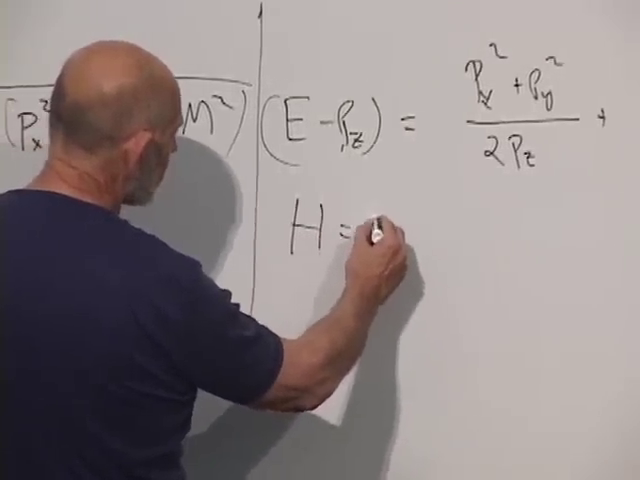
\includegraphics[width=\textwidth]{lecture_02_figure_02.png}
    \par\smallskip\footnotesize (a) 端點固定且斜率為零的形狀。
  \end{minipage}\hfill
  \begin{minipage}[t]{0.48\textwidth}
    \centering
    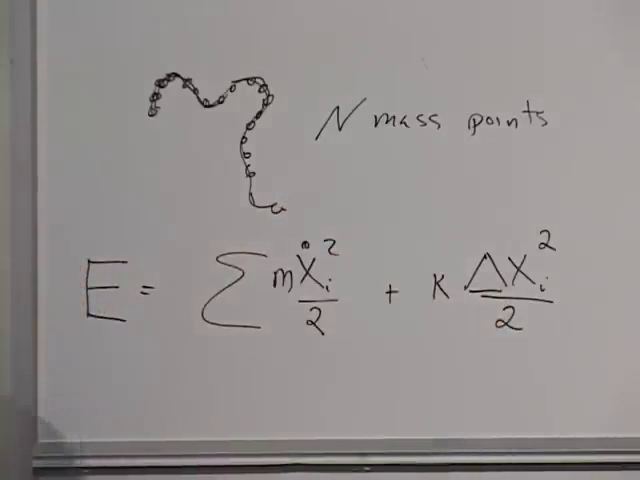
\includegraphics[width=\textwidth]{lecture_02_figure_03.png}
    \par\smallskip\footnotesize (b) 在豎直桿上滑動的輕環。
  \end{minipage}
  \caption{以形狀與力學呈現邊界條件。滑環模型明確描述了自由端點的橫向運動。}
  \lectureframe{00:08:50 and 00:12:15}
  \label{fig:l02-boundaries-board}
\end{figure}

\begin{figure}[H]
  \centering
  \begin{adjustbox}{max width=\linewidth}
  \begin{tikzpicture}[>=Latex,thick,scale=0.92]
    \begin{scope}
      \draw[->] (0,0) -- (4.4,0) node[right] {\(\sigma\)};
      \draw[->] (0,-1.25) -- (0,1.35) node[above] {\(x\)};
      \draw[blue!70!black]
        (0,0) .. controls (0.8,1.1) and (1.4,1.0) .. (2.0,0)
        .. controls (2.7,-1.0) and (3.4,-0.8) .. (4.1,0);
      \fill (0,0) circle (0.06);
      \fill (4.1,0) circle (0.06);
      \node at (2.05,-1.65) {Dirichlet: \(x=0\)};
    \end{scope}
    \begin{scope}[xshift=5.8cm]
      \draw[->] (0,0) -- (4.4,0) node[right] {\(\sigma\)};
      \draw[->] (0,-1.25) -- (0,1.35) node[above] {\(x\)};
      \draw[orange!85!black]
        (0,0.65) .. controls (0.8,0.65) and (1.1,-0.9) .. (2.0,-0.9)
        .. controls (2.9,-0.9) and (3.2,0.55) .. (4.1,0.55);
      \draw[orange!85!black] (0,0.65) -- (0.45,0.65);
      \draw[orange!85!black] (3.65,0.55) -- (4.1,0.55);
      \node at (2.05,-1.65) {Neumann: \(\partial_\sigma x=0\)};
    \end{scope}
  \end{tikzpicture}
  \end{adjustbox}
  \caption{狄利克雷條件固定函數值；諾伊曼條件固定斜率。}
  \label{fig:l02-boundaries-redraw}
\end{figure}

\begin{classroomqa}
\audiencequestion{開管或閉管風琴能否作為其中一種邊界條件的明確例子？\lecturetimestamp{00:09:19}}
\lecturerresponse{可以，但首先必須說明要展開的是哪個聲學變數。在理想化情況下，開口端的壓力擾動與縱向位移滿足互補的條件。與其在黑板上處理這個旁枝問題，不如採用滑環模型：近乎無質量的環能沿桿上下滑動，因此弦的端點是自由的，諾伊曼條件也一目了然。}
\end{classroomqa}

\begin{classroomqa}
\audiencequestion{圖形能否垂直上升，並包含尖銳的跳躍？\lecturetimestamp{00:09:53}}
\lecturerresponse{傅立葉分析容許分段連續函數有孤立跳躍，但物理弦受到更嚴格的限制。跳躍會使相鄰點斷開，並使空間導數 \(\partial_\sigma x\) 在下文推導的連續能量中變得奇異。因此，我們只考慮連續且可微的形狀。}
\end{classroomqa}

\begin{classroomqa}
\audiencequestion{為什麼管子的開口端，或任何自由端，都必須滿足邊界條件？\lecturetimestamp{00:11:14}}
\lecturerresponse{聲學例子取決於所選的場變數，講解中沒有進一步處理。力學例子則不同。極輕的環可以自由滑動，但仍與弦的最後一段相連。我們不預設端點條件，而是從牛頓定律推導：要使端點加速度有限，斜率就必須為零。}
\end{classroomqa}

\subsection{傅立葉基底}

端點條件的類別一旦確定，相應的傅立葉基底也就確定。在 \(0\leq\sigma\leq\pi\) 上，

\begin{align}
  x_D(\sigma)
  &=
  \sum_{n=1}^{\infty}x_n\sin(n\sigma),
  \label{eq:l02-dirichlet-series}\\
  x_N(\sigma)
  &=
  \sum_{n=0}^{\infty}x_n\cos(n\sigma).
  \label{eq:l02-neumann-series}
\end{align}

\eqref{eq:l02-dirichlet-series} 中的每個正弦函數在兩個端點都為零。
\eqref{eq:l02-neumann-series} 中的每個餘弦函數在端點處的導數都為零。
求和下限不同是有原因的：
\(\sin(0\sigma)=0\) 不會有貢獻，而
\(\cos(0\sigma)=1\) 是常數模態，也就是零模態。它代表諾伊曼函數的平均值。

\begin{figure}[H]
  \centering
  \begin{minipage}[t]{0.48\textwidth}
    \centering
    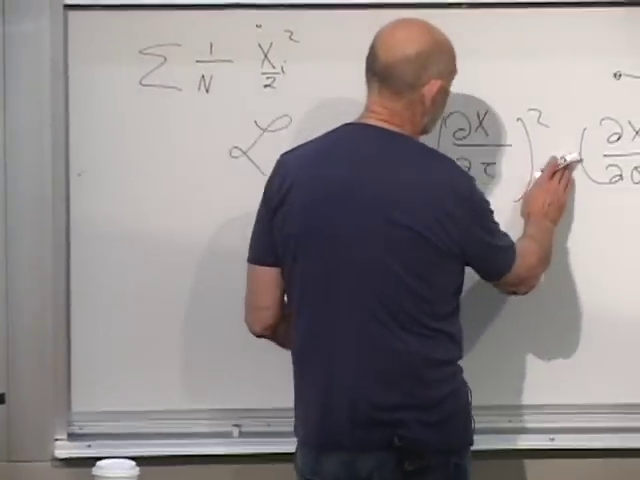
\includegraphics[width=\textwidth]{lecture_02_figure_04.png}
    \par\smallskip\footnotesize (a) 正弦與餘弦展開。
  \end{minipage}\hfill
  \begin{minipage}[t]{0.48\textwidth}
    \centering
    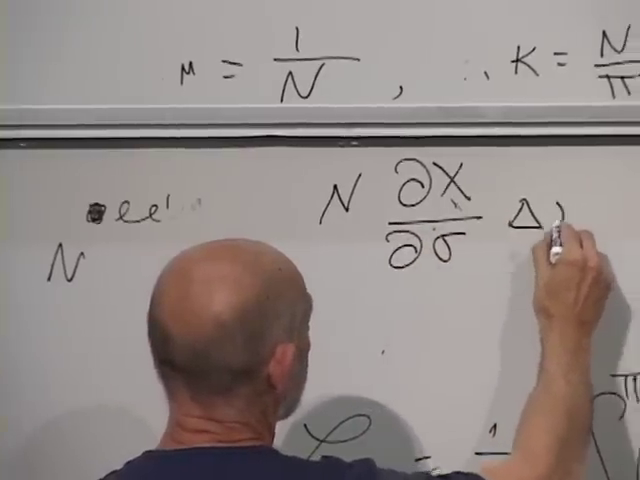
\includegraphics[width=\textwidth]{lecture_02_figure_05.png}
    \par\smallskip\footnotesize (b) 正交性與例外的
    常數模態。
  \end{minipage}
  \caption{後續將用來對角化弦的傅立葉性質。}
  \lectureframe{00:16:15 and 00:20:30}
  \label{fig:l02-fourier-board}
\end{figure}

微分會使這兩類互相轉換：

\begin{equation}
  \begin{aligned}
    \partial_\sigma\sin(n\sigma)&=n\cos(n\sigma),\\
    \partial_\sigma\cos(n\sigma)&=-n\sin(n\sigma).
  \end{aligned}
  \label{eq:l02-basis-derivatives}
\end{equation}

因此，狄利克雷級數的導數具有諾伊曼型態，而諾伊曼級數的導數則具有狄利克雷型態。接著，正交性會消去不同模態間的交叉項：

\begin{align}
  \int_0^\pi\cos(n\sigma)\cos(m\sigma)\,d\sigma
  &=
  \frac{\pi}{2}\delta_{nm},
  && n,m\geq1,
  \label{eq:l02-cos-orthogonality}\\
  \int_0^\pi\sin(n\sigma)\sin(m\sigma)\,d\sigma
  &=
  \frac{\pi}{2}\delta_{nm},
  && n,m\geq1,
  \label{eq:l02-sin-orthogonality}\\
  \int_0^\pi 1\,d\sigma&=\pi .
  \label{eq:l02-zero-norm}
\end{align}

最後一行是例外的 \(n=m=0\) 餘弦範數。常數模態的歸一化方式不同於非零諧波；這個二倍因子將區分弦的質心模態與內部模態。

\subsection{要記住的一個振子公式}

將座標重新標度，使其力學質量為一後，遵循虎克定律的振子具有

\begin{align}
  E_{\mathrm{osc}}
  &=
  \frac12\dot q^{\,2}
  +\frac12\omega^2q^2,
  \label{eq:l02-oscillator-energy}\\
  L_{\mathrm{osc}}
  &=
  \frac12\dot q^{\,2}
  -\frac12\omega^2q^2.
  \label{eq:l02-oscillator-lagrangian}
\end{align}

\begin{figure}[H]
  \centering
  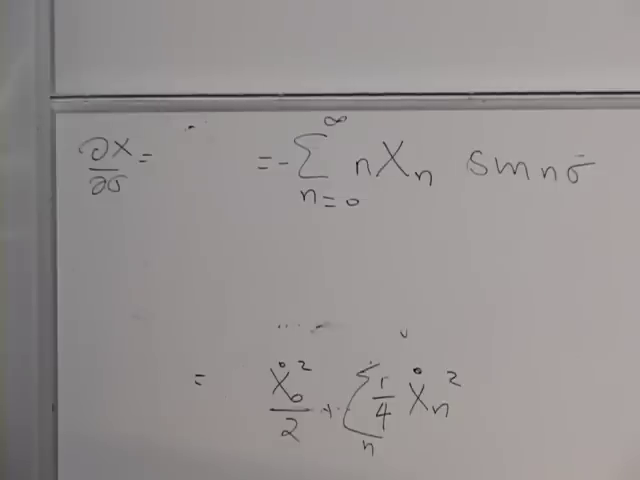
\includegraphics[width=0.68\textwidth]{lecture_02_figure_06.png}
  \caption{振子的能量寫成這個形式後，\(q^2\) 的係數便能
  直接看出 \(\omega^2\)。}
  \lectureframe{00:24:00}
  \label{fig:l02-oscillator-board}
\end{figure}

在經典力學中，\(\omega=\sqrt{\kappa/m}\)；座標重新標度後，\(m=1\)。在量子力學中，

\begin{equation}
  E_Q=\hbar\omega\left(Q+\frac12\right),
  \qquad Q=0,1,2,\ldots .
  \label{eq:l02-oscillator-spectrum}
\end{equation}

討論能級間距時，可以扣除各能級共有的基態能量，並說每個量子所需的能量為 \(\hbar\omega\)。弦的計算一開始也會這麼做，總零點能則留待之後處理。

\begin{classroomqa}
\audiencequestion{如何從能量公式看出振子的頻率？\lecturetimestamp{00:23:21}}
\lecturerresponse{重新標度之前，頻率為
\(\omega=\sqrt{\kappa/m}\)。質量設為一時，勢能項為
\(\frac12\omega^2q^2\)，因此它的二次項係數就是頻率的平方。}
\end{classroomqa}

\section{複合系統在什麼意義上算是粒子？}

弦具有延展性，我們會以許多彼此耦合的部分來建模。那麼，它的一個量子態在什麼意義上仍可稱為粒子？點狀性不能作為決定性判據。質子與中子都是複合粒子。電子與光子也受到量子場的修飾，儘管尚未測得其內在子結構。周圍空無一物的經典幾何點，並不是量子激發的恰當圖像。

光有質量與質心位置也不足以構成判據。密封的氣體箱兩者兼具，一杯咖啡也一樣；我們通常不會把它們稱為粒子。不可分性同樣不是判據，因為質子可以分解；自旋也無法區分微觀粒子與宏觀物體。

有用的判據是能譜是否隔離。將靜止能量標在縱軸上，再問要增加多少能量才能到達另一個內部態。電子附近沒有實驗可及的電子激發態序列。質子則有共振態，但最低幾個共振態所需能量達數百 MeV，約為質子質量的相當一部分。這些態彼此分隔得夠遠，因此能逐一辨識。

一杯咖啡的情形正好相反。只要加入任意微小的能量，就能激發長波長聲模態、推動分子，或產生聲子。極大量的態密集分布在極小的能量區間內；在實驗室尺度上，它們構成連續譜。這就是粒子與\emph{一團混沌}之間實際上的差別。

\begin{figure}[H]
  \centering
  \includegraphics[width=0.58\textwidth]{lecture_02_figure_07.png}
  \caption{比較孤立的粒子能級與普通物質密集的激發態時，黑板上的縱向能量軸。}
  \lectureframe{00:31:10}
  \label{fig:l02-spectrum-board}
\end{figure}

\begin{figure}[H]
  \centering
  \begin{adjustbox}{max width=\linewidth}
  \begin{tikzpicture}[>=Latex,thick]
    \begin{scope}
      \draw[->] (0,0) -- (0,4.8) node[above] {energy};
      \draw[blue!70!black,line width=1.2pt] (-1.0,0.65) -- (1.0,0.65);
      \draw[blue!70!black,line width=1.2pt] (-1.0,3.65) -- (1.0,3.65);
      \node[right] at (1.05,0.65) {ground state};
      \node[right] at (1.05,3.65) {first internal excitation};
      \draw[<->] (0.65,0.75) -- (0.65,3.55)
        node[midway,right] {large gap};
      \node at (0,-0.55) {particle-like};
    \end{scope}
    \begin{scope}[xshift=7.0cm]
      \draw[->] (0,0) -- (0,4.8) node[above] {energy};
      \foreach \y in {0.55,0.69,0.82,0.94,1.05,1.15,1.24,1.32,1.39,1.45,
        1.51,1.57,1.63,1.70,1.78,1.87,1.97,2.09,2.22,2.36,2.51,2.67,2.84,
        3.02,3.21,3.41,3.62,3.84,4.07}
        \draw[orange!85!black] (-0.95,\y) -- (0.95,\y);
      \node[right] at (1.05,2.25) {dense phonon and internal states};
      \node at (0,-0.55) {macroscopic matter};
    \end{scope}
  \end{tikzpicture}
  \end{adjustbox}
  \caption{講座採用的操作性粒子判據是能譜隔離，而非字面上的點狀性。}
  \label{fig:l02-particle-redraw}
\end{figure}

這項判據將哲學問題轉化為計算：量子化弦，找出它的內部能級，再檢視能級間距。如果弦的第一激發態位於普朗克尺度附近，而觀測到的基態質量很小，那麼兩者間的能隙就比目前加速器所能達到的能量高出二十多個數量級。在所有可及的能量範圍內，弦因此都會呈現基本粒子的行為。

\begin{classroomqa}
\audiencequestion{粒子行為只是觀測尺度的問題嗎？如果放大到足夠大的程度，能級會不再彼此分離嗎？\lecturetimestamp{00:33:33}}
\lecturerresponse{放大可能揭露物體由許多組分構成，但不會消除它的能譜。關鍵在於比較實驗的能量解析度與第一個內部激發態的能隙。只要能隙極大，複合物體仍可能呈現粒子般的行為。}
\end{classroomqa}

\begin{classroomqa}
\audiencequestion{為什麼普通的小提琴弦不是粒子？\lecturetimestamp{00:34:37}}
\lecturerresponse{一個振動量子所帶的能量，與宏觀弦的靜止能量相比小得無法測量。因此，在極小的相對能量區間內就有許多量子態。它屬於能譜比較中密集的一側，而非孤立的一側。}
\end{classroomqa}

\begin{classroomqa}
\audiencequestion{如果量子場以虛擬漲落修飾光子與電子，它們還算是點粒子嗎？\lecturetimestamp{00:35:40}}
\lecturerresponse{經典意義下的\emph{點}這個詞承載了太多含義。實際的電子與光子是受到場修飾的激發態，但實驗尚未發現它們具有內在組分結構或有限的形狀因子。就目前的論證而言，重點是兩者都沒有密集、近乎簡併的內部態序列。\editorialnote{講座將電子的反常磁矩與可測量的量子模糊性聯繫起來。以現代術語來說，反常磁矩是輻射修飾效應，並非電子具有可分辨有限半徑的證據。依照慣例，所謂點狀，是指在已測試的尺度內尚未探測到內在子結構或形狀因子。}}
\end{classroomqa}

\begin{classroomqa}
\audiencequestion{光子的大小會隨頻率改變嗎？\lecturetimestamp{00:36:49}}
\lecturerresponse{光子的波長確實取決於頻率，但那與內在的組分大小不同。改變頻率會改變波包與波長，不會改變光子可分辨的內部半徑。}
\end{classroomqa}

\section{大動量下的精確橫向力學}

現在回到相對論帶來的困難。不能只把快速旋轉的短棒質心置於靜止，就將它視為非相對論系統；短棒兩端彼此之間仍作相對論性運動。非相對論近似失效的原因，是系統內部存在相對運動。

然而，還有另一種極限。選定 \(z\) 軸，並對整個系統沿該軸作洛倫茲 boost，使縱向動量 \(P_z\) 變得極大。保持其橫向動量

\begin{equation}
  p_\perp^2=p_x^2+p_y^2
\end{equation}

有限。在 \(P_z\to\infty\) 的極限下，橫向投影可精確寫成非相對論哈密頓量的形式，即使 boost 前的內部運動原本具有相對論性。

\begin{classroomqa}
\audiencequestion{無限動量是否代表有質量的系統實際上達到了光速？\lecturetimestamp{00:40:43}}
\lecturerresponse{任何有限的 boost 都無法使它達到光速。我們所構造的是在 \(P_z\) 任意增大時具有良好定義極限的物理量。這個說法指的是一種取極限的程序，而不是具有 \(v=c\) 的有限物理狀態。}
\end{classroomqa}

\begin{classroomqa}
\audiencequestion{應該選哪個軸？如果物體繞著該軸旋轉，或在垂直於該軸的方向上運動，又會如何？\lecturetimestamp{00:41:14}}
\lecturerresponse{可以選擇任意軸，並沿該軸對整個系統作 boost。明確保留下來的力學，是物體在垂直平面上的投影。一根旋轉的桿可能看起來縮短了，也可能掃過該平面，但它的橫向投影仍具有非相對論形式。}
\end{classroomqa}

弦還有一項性質，使這種描述格外有力。在光前規範中，弦的縱向內部座標不是獨立的振子，而是由約束根據橫向運動決定。因此，只要知道弦的橫向狀態，就足以重建其物理自由度。

\begin{classroomqa}
\audiencequestion{沒有獨立的縱向座標，是否代表弦只是被困在一個薄薄的夾層中？\lecturetimestamp{00:42:26}}
\lecturerresponse{洛倫茲收縮確實會使弦在 boost 後參考系中的縱向延展變小，但這裡的論述更強。任何剩餘的縱向運動都受橫向運動約束，不能獨立指定。}
\end{classroomqa}

\begin{classroomqa}
\audiencequestion{這種將描述化約為橫向資料的做法，與全息原理有關嗎？\lecturetimestamp{00:43:12}}
\lecturerresponse{它與促成全息思想的思路密切相關，不過探討這項關聯會使我們偏離目前的計算。在此處，這項關聯只用來說明為何可以只處理弦的橫向部分。}
\end{classroomqa}

\subsection{扣除 boost 能量並重新標度時間}

設 \(M\) 為整個系統的不變質量，包含組分質量、動能與束縛能。在 \(c=1\) 單位制下，

\begin{equation}
  E=\sqrt{P_z^2+p_\perp^2+M^2}.
  \label{eq:l02-relativistic-energy}
\end{equation}

當 \(P_z\) 遠大於 \(p_\perp\) 與 \(M\) 時，

\begin{equation}
  E
  =
  P_z+\frac{p_\perp^2+M^2}{2P_z}
  +O(P_z^{-3}).
  \label{eq:l02-large-pz}
\end{equation}

\begin{figure}[H]
  \centering
  \includegraphics[width=0.76\textwidth]{lecture_02_figure_08.png}
  \caption{完整的高 \(P_z\) 展開式，保留了橫向動量與不變質量。}
  \lectureframe{00:47:30}
  \label{fig:l02-large-pz-board}
\end{figure}

領先項很大，卻不含任何內部狀態的資訊。若過程中 \(P_z\) 守恆，例如受 boost 的原子在總縱向動量不變時於內部能級間躍遷，這一項就會從所有能量差中抵消。因此我們研究

\begin{equation}
  E-P_z=\frac{p_\perp^2+M^2}{2P_z}+O(P_z^{-3}).
  \label{eq:l02-residual-energy}
\end{equation}

分母具有物理意義。哈密頓量生成時間演化，因此微小的剩餘能量表示內部演化在實驗室時間中看來較慢，這就是時間膨脹。若要保留內部運動，可引入重新標度後的演化參數 \(\tau\)，或等價地將剩餘哈密頓量乘以 \(P_z\)：

\begin{equation}
  H_\perp
  \equiv
  \lim_{P_z\to\infty}P_z(E-P_z)
  =
  \frac12p_\perp^2+\frac12M^2.
  \label{eq:l02-transverse-hamiltonian}
\end{equation}

\begin{figure}[H]
  \centering
  \begin{minipage}[t]{0.48\textwidth}
    \centering
    \includegraphics[width=\textwidth]{lecture_02_figure_09.png}
    \par\smallskip\footnotesize (a) \(H=i\partial_t\) 與變慢的內部
    演化。
  \end{minipage}\hfill
  \begin{minipage}[t]{0.48\textwidth}
    \centering
    \includegraphics[width=\textwidth]{lecture_02_figure_10.png}
    \par\smallskip\footnotesize (b) 重新標度時間後的有限橫向哈密頓量。
  \end{minipage}
  \caption{從因時間膨脹而變小的剩餘能量，得到有限的
  二維哈密頓量。}
  \lectureframe{00:49:20 and 00:52:40}
  \label{fig:l02-lightfront-board}
\end{figure}

這正是單位質量粒子在二維中運動的形式：動能 \(p_\perp^2/2\) 加上內部能量 \(M^2/2\)。特別之處在於平方項。在這種描述中，扮演靜止能量或束縛能角色的量，正比於不變質量的平方。\editorialnote{採用傳統的光前變數 \(P^\pm=(E\pm P_z)/\sqrt2\) 時，精確的質殼關係為 \(2P^+P^-=p_\perp^2+M^2\)。方程 \eqref{eq:l02-transverse-hamiltonian} 則是本講以高 \(P_z\) 為基準正規化後的同一不變關係。}

\begin{classroomqa}
\audiencequestion{複合系統中各個組成部分的縱向動量去哪裡了？\lecturetimestamp{00:51:30}}
\lecturerresponse{一般的複合物體必須保留各組分所帶總 \(P_z\) 的比例。上面的公式使用的是總質心動量。弦論的特殊之處，在於其約束可由橫向自由度決定相對縱向運動，因此不必另外加入獨立的縱向振子。}
\end{classroomqa}

\section{離散開弦}

現在，弦明確地只在橫向平面中運動。將兩個座標標記為 \(X\) 與 \(Y\)，並先以 \(N\) 個質點和連接它們的 \(N-1\) 根彈簧近似弦。若 \(\mu\) 是每個質點的類比質量，而 \(k\) 是最近鄰彈簧常數，則能量為

\begin{equation}
  E_N
  =
  \sum_i
  \left[
    \frac{\mu}{2}
    \left(\dot X_i^2+\dot Y_i^2\right)
    +
    \frac{k}{2}
    \left((\Delta X_i)^2+(\Delta Y_i)^2\right)
  \right].
  \label{eq:l02-discrete-energy}
\end{equation}

每個 \(X\) 項都有一個相同的 \(Y\) 項，因為橫向平面有兩個方向。指標 \(i\) 標示鏈上的點，並非空間座標。

\begin{figure}[H]
  \centering
  \begin{minipage}[t]{0.48\textwidth}
    \centering
    \includegraphics[width=\textwidth]{lecture_02_figure_11.png}
    \par\smallskip\footnotesize (a) 質點鏈及其離散能量。
  \end{minipage}\hfill
  \begin{minipage}[t]{0.48\textwidth}
    \centering
    \includegraphics[width=\textwidth]{lecture_02_figure_12.png}
    \par\smallskip\footnotesize (b) \(N\) 增大時 \(\mu\) 與 \(k\) 的標度變化。
  \end{minipage}
  \caption{取連續極限前的正則化開弦。}
  \lectureframe{00:57:42 and 01:02:40}
  \label{fig:l02-chain-board}
\end{figure}

\begin{figure}[H]
  \centering
  \begin{adjustbox}{max width=\linewidth}
  \begin{tikzpicture}[>=Latex,thick]
    \foreach \i in {0,...,8} {
      \coordinate (p\i) at ({1.05*\i},{0.30*sin(55*\i)});
      \filldraw[white] (p\i) circle (0.10);
      \draw (p\i) circle (0.10);
    }
    \foreach \i in {0,...,7} {
      \pgfmathtruncatemacro{\j}{\i+1}
      \draw[decorate,decoration={zigzag,segment length=4pt,amplitude=2pt}]
        (p\i) -- (p\j);
    }
    \node[above=0.35cm of p0] {\(i=0\)};
    \node[above=0.35cm of p8] {\(i=N-1\)};
    \draw[<->] (0,-1.15) -- (8.4,-1.15)
      node[midway,below] {\(0\leq\sigma\leq\pi\)};
    \node at (4.2,1.25)
      {\(\mu=1/N,\quad k=N/\pi^2,\quad\Delta\sigma=\pi/N\)};
  \end{tikzpicture}
  \end{adjustbox}
  \caption{清楚的正則化示意圖。鏈逐漸細分時，質點會變輕，而微觀彈簧會變硬。}
  \label{fig:l02-chain-redraw}
\end{figure}

參數 \(\sigma\) 標示沿鏈的位置。選擇 \(0\leq\sigma\leq\pi\) 是一種約定，並非對物理長度的測量。這提醒我們弦有兩個端點。稍後，閉弦的位置將以 \(0\leq\sigma<2\pi\) 為週期標記。

連續極限必須使整體力學量保持有限。若每個質點的質量固定，總類比質量就會發散，因此取

\begin{equation}
  \mu=\frac{1}{N}.
  \label{eq:l02-mu-scaling}
\end{equation}

於是 \(N\mu=1\)。這不是相對論中的靜止質量 \(M\)，而是橫向類比模型中的慣性係數。

串聯彈簧的數目增加時，整體會變軟。若要使整條鏈的勁度保持有限，每根微觀彈簧就必須變硬：

\begin{equation}
  k=\frac{N}{\pi^2}
  =\frac{1}{\pi\,\Delta\sigma}.
  \label{eq:l02-k-scaling}
\end{equation}

只有 \(k\propto N\) 是必要的。因子 \(\pi^2\) 是一種正規化選擇，用來從連續公式中消除多餘的 \(\pi\) 因子。

\begin{classroomqa}
\audiencequestion{\(\mu\) 是每個弦點的物理靜止質量嗎？\lecturetimestamp{01:10:34}}
\lecturerresponse{不是。它是橫向質點鏈中的非相對論類比質量。稱它為 \(M\)，會使人將它與整個相對論弦態的不變靜止質量混淆。它在此處的唯一用途，是產生正確的連續極限慣性。}
\end{classroomqa}

\section{連續波動系統}

套用開頭整理好的規則。由於
\(1/N=\Delta\sigma/\pi\)，

\begin{align}
  \sum_i\frac{\mu}{2}\dot X_i^2
  &=
  \frac{1}{2\pi}
  \sum_i\dot X_i^2\,\Delta\sigma
  \longrightarrow
  \frac{1}{2\pi}
  \int_0^\pi
  \left(\partial_\tau X\right)^2d\sigma ,
  \label{eq:l02-kinetic-limit}\\
  \sum_i\frac{k}{2}(\Delta X_i)^2
  &\longrightarrow
  \frac{1}{2\pi}
  \int_0^\pi
  \left(\partial_\sigma X\right)^2d\sigma .
  \label{eq:l02-potential-limit}
\end{align}

第二行使用
\(\Delta X_i=\partial_\sigma X\,\Delta\sigma\) 以及
\(k=1/(\pi\Delta\sigma)\)。對 \(Y\) 也可作相同計算。

\begin{figure}[H]
  \centering
  \begin{minipage}[t]{0.48\textwidth}
    \centering
    \includegraphics[width=\textwidth]{lecture_02_figure_13.png}
    \par\smallskip\footnotesize (a) 將總和轉為積分，並將
    差分轉為導數。
  \end{minipage}\hfill
  \begin{minipage}[t]{0.48\textwidth}
    \centering
    \includegraphics[width=\textwidth]{lecture_02_figure_14.png}
    \par\smallskip\footnotesize (b) 完成連續極限後的能量。
  \end{minipage}
  \caption{離散鏈在 \(\sigma\) 區間上轉變為場。}
  \lectureframe{01:05:40 and 01:07:00}
  \label{fig:l02-continuum-board}
\end{figure}

因此得到的能量與拉格朗日量為

\begin{align}
  E
  &=
  \frac{1}{2\pi}
  \int_0^\pi d\sigma\,
  \left[
    (\partial_\tau X)^2+(\partial_\tau Y)^2\right.\notag\\[-0.25em]
  &\hspace{6.5em}\left.
    +(\partial_\sigma X)^2+(\partial_\sigma Y)^2
  \right],
  \label{eq:l02-continuum-energy}\\
  L
  &=
  \frac{1}{2\pi}
  \int_0^\pi d\sigma\,
  \left[
    (\partial_\tau X)^2+(\partial_\tau Y)^2\right.\notag\\[-0.25em]
  &\hspace{6.5em}\left.
    -(\partial_\sigma X)^2-(\partial_\sigma Y)^2
  \right].
  \label{eq:l02-continuum-lagrangian}
\end{align}

\begin{figure}[H]
  \centering
  \includegraphics[width=0.78\textwidth]{lecture_02_figure_15.png}
  \caption{連續極限下的拉格朗日量，其中動能項與拉伸項
  的符號相反。}
  \lectureframe{01:08:48}
  \label{fig:l02-lagrangian-board}
\end{figure}

若將 \(\sigma\) 改稱為一般的空間座標，並將 \(X\) 改稱為場 \(\phi\)，這些就是一維波場的能量與拉格朗日量。對 \eqref{eq:l02-continuum-lagrangian} 作變分，得到

\begin{equation}
  \left(\partial_\tau^2-\partial_\sigma^2\right)X=0,
  \qquad
  \left(\partial_\tau^2-\partial_\sigma^2\right)Y=0.
  \label{eq:l02-wave-equation}
\end{equation}

眼前的論證不需要直接求解這些方程。只要掌握以下圖像即可：波沿弦向左、向右傳播，並在端點反射。狄利克雷反射會使位移反號；諾伊曼反射則保持位移的符號。

\begin{classroomqa}
\audiencequestion{時間變數 \(\tau\) 究竟是什麼？\lecturetimestamp{01:08:54}}
\lecturerresponse{它是在高 \(P_z\) 描述中追蹤內部運動的重新標度時間。與系統一同受 boost 的時鐘相較於實驗室時鐘走得較慢；\(\tau\) 可消除這種時間膨脹，使內部振盪維持有限的頻率。對這裡討論的橫向力學而言，可以直接把它當作時間。\editorialnote{講義非正式地將 \(\tau\) 稱為固有時。對延展的弦而言，精確的光前演化參數是經過規範固定的重新標度時間，而不是所有弦上位置共用的單一不變固有時。這不影響原本的時間膨脹論證。}}
\end{classroomqa}

當質心在橫向平面中靜止時，\eqref{eq:l02-continuum-energy} 的內部部分，依照 \eqref{eq:l02-transverse-hamiltonian} 的正規化，正比於 \(M^2\)。因此，量子化這個表面上尋常的波動系統，就能揭示相對論性的質量譜。

\begin{classroomqa}
\audiencequestion{\(P_z(E-P_z)\) 有名稱嗎？\lecturetimestamp{01:11:00}}
\lecturerresponse{它通常稱為光錐能量或光前能量。「光前」更能描述作為演化曲面的零平面；採用哪個傳統術語，並不影響計算。}
\end{classroomqa}

\begin{classroomqa}
\audiencequestion{「錐」是指一般時空中的光錐嗎？這個術語是 Dirac 提出的嗎？\lecturetimestamp{01:11:17}}
\lecturerresponse{零座標的構造可以用 45 度軸繪出，但此處的演化曲面是光前，而非完整的膨脹光錐。Dirac 曾發展相關的相對論動力學形式；至於名稱的歷史由來，講解中並未定論，也不影響方程。}
\end{classroomqa}

\section{為什麼自由端點滿足諾伊曼條件}

現在可以推導端點條件，而不必預先假設。由於經過 boost 的橫向力學恰好具有非相對論形式，因此可以使用牛頓定律。內部質點受到兩側彈簧的拉力；末端質點則只受到連接相鄰質點的那根彈簧拉力。

\begin{classroomqa}
\audiencequestion{討論相對論性弦時，為什麼可以使用牛頓定律？\lecturetimestamp{01:14:52}}
\lecturerresponse{我們並非將牛頓力學用於未經 boost 的完整時空運動，而是用於無限動量描述中的橫向變數；這些變數的哈密頓量恰好具有非相對論形式。}
\end{classroomqa}

在右端點，依虎克定律，力為（正負號取決於方向）

\begin{equation}
  F_{\mathrm{end}}
  =
  -k\,\Delta X
  =
  -\frac{1}{\pi\Delta\sigma}
   \left(\partial_\sigma X\,\Delta\sigma\right)
  =
  -\frac{1}{\pi}\partial_\sigma X .
  \label{eq:l02-endpoint-force}
\end{equation}

\begin{figure}[H]
  \centering
  \begin{minipage}[t]{0.48\textwidth}
    \centering
    \includegraphics[width=\textwidth]{lecture_02_figure_16.png}
    \par\smallskip\footnotesize (a) 端點受力與當地
    斜率成正比。
  \end{minipage}\hfill
  \begin{minipage}[t]{0.48\textwidth}
    \centering
    \includegraphics[width=\textwidth]{lecture_02_figure_17.png}
    \par\smallskip\footnotesize (b) 有限加速度條件。
  \end{minipage}
  \caption{以牛頓定律推導自由端的邊界條件。}
  \lectureframe{01:18:20 and 01:20:10}
  \label{fig:l02-neumann-board}
\end{figure}

末端質點的牛頓運動方程為

\begin{equation}
  \mu\,\partial_\tau^2X=F_{\mathrm{end}},
  \qquad
  \mu=\frac1N=\frac{\Delta\sigma}{\pi}.
  \label{eq:l02-endpoint-newton}
\end{equation}

合併 \eqref{eq:l02-endpoint-force} 與
\eqref{eq:l02-endpoint-newton}，

\begin{equation}
  \partial_\sigma X
  =
  -\Delta\sigma\,\partial_\tau^2X
  \quad\text{at the right endpoint},
  \label{eq:l02-endpoint-scaling}
\end{equation}

左端點的受力方向相反。若 \(\partial_\sigma X\) 在
\(\Delta\sigma\to0\) 時趨近非零常數，端點加速度就會如 \(N\) 般發散。
因此，要使連續極限合理且加速度有限，就必須有

\begin{equation}
  \left.\partial_\sigma X\right|_{0,\pi}=0,
  \qquad
  \left.\partial_\sigma Y\right|_{0,\pi}=0.
  \label{eq:l02-open-neumann}
\end{equation}

\begin{figure}[H]
  \centering
  \begin{adjustbox}{max width=\linewidth}
  \begin{tikzpicture}[>=Latex,thick,scale=1.0]
    \coordinate (a) at (0,0);
    \coordinate (b) at (4.5,0.75);
    \filldraw[white] (a) circle (0.12);
    \draw (a) circle (0.12);
    \filldraw[white] (b) circle (0.12);
    \draw (b) circle (0.12);
    \draw[decorate,decoration={zigzag,segment length=6pt,amplitude=3pt}]
      (a) -- (b);
    \draw[dashed] (a) -- (0,-1.2);
    \draw[dashed] (b) -- (4.5,-1.2);
    \draw[<->] (4.85,0) -- (4.85,0.75)
      node[midway,right] {\(\Delta X\)};
    \draw[->,red!70!black] (b) -- (5.75,0.95)
      node[right] {\(F_{\rm end}=-k\Delta X\)};
    \node[below] at (0,-1.2) {\(N-1\)};
    \node[below] at (4.5,-1.2) {\(N\)};
    \node at (2.5,-2.0)
      {\(\mu\ddot X=-k\Delta X
      \ \Longrightarrow\
      \partial_\sigma X=-\Delta\sigma\,\ddot X\to0\)};
  \end{tikzpicture}
  \end{adjustbox}
  \caption{在正則化極限下，末端質點的質量趨近於零。只有端點斜率趨近於零，
  加速度才可能有限。}
  \label{fig:l02-neumann-redraw}
\end{figure}

對兩端與兩個橫向方向作相同論證，就得到自由開弦的諾伊曼邊界條件。

\section{開弦的簡正模態}

現在我們已經得到完整的古典系統，包括拉格朗日量與邊界條件。經過傅立葉分析後，量子化就變得簡單。由於端點滿足諾伊曼條件，

\begin{align}
  X(\sigma,\tau)
  &=
  \sum_{n=0}^{\infty}X_n(\tau)\cos(n\sigma),
  \label{eq:l02-X-expansion}\\
  Y(\sigma,\tau)
  &=
  \sum_{n=0}^{\infty}Y_n(\tau)\cos(n\sigma).
  \label{eq:l02-Y-expansion}
\end{align}

所有 \(\sigma\) 依賴都包含在餘弦函數中；所有時間依賴則包含在係數中。\(X_n(\tau)\) 與 \(Y_n(\tau)\) 隨時間改變，弦也因此振動。

\begin{figure}[H]
  \centering
  \includegraphics[width=0.78\textwidth]{lecture_02_figure_18.png}
  \caption{尼曼模態展開式與將使雙重求和化簡的正交關係並列。}
  \lectureframe{01:21:45}
  \label{fig:l02-mode-expansion-board}
\end{figure}

\subsection{動能項與零模}

對時間微分可得

\begin{equation}
  \partial_\tau X
  =
  \sum_{n=0}^{\infty}\dot X_n(\tau)\cos(n\sigma).
  \label{eq:l02-time-mode}
\end{equation}

平方後會得到對 \(n\) 和 \(m\) 的雙重求和，但
\eqref{eq:l02-cos-orthogonality}會消去所有滿足 \(n\neq m\) 的項。
將常數模另行處理，

\begin{equation}
  \frac{1}{2\pi}\int_0^\pi
  (\partial_\tau X)^2\,d\sigma
  =
  \frac12\dot X_0^{\,2}
  +
  \frac14\sum_{n=1}^{\infty}\dot X_n^{\,2}.
  \label{eq:l02-mode-kinetic}
\end{equation}

\begin{figure}[H]
  \centering
  \includegraphics[width=0.76\textwidth]{lecture_02_figure_19.png}
  \caption{正交性積分將動能的雙重求和化為零模項與對角求和。}
  \lectureframe{01:29:10}
  \label{fig:l02-mode-kinetic-board}
\end{figure}

常數係數就是平均位置，

\begin{equation}
  X_0(\tau)=\frac1\pi\int_0^\pi X(\sigma,\tau)\,d\sigma ,
  \label{eq:l02-center-of-mass}
\end{equation}

對 \(Y_0\) 也一樣。在均勻的類比質量密度下，這些就是質心座標。它們具有動能，卻沒有恢復力：整條弦可以在橫向平面中自由移動。

\subsection{拉伸項與振子頻率}

對空間微分可得

\begin{equation}
  \partial_\sigma X
  =
  -\sum_{n=1}^{\infty}nX_n(\tau)\sin(n\sigma).
  \label{eq:l02-spatial-mode}
\end{equation}

零模消失了，因為均勻平移不會拉伸弦。利用正弦函數的正交性，

\begin{equation}
  \frac{1}{2\pi}\int_0^\pi
  (\partial_\sigma X)^2\,d\sigma
  =
  \frac14\sum_{n=1}^{\infty}n^2X_n^{\,2}.
  \label{eq:l02-mode-potential}
\end{equation}

\begin{figure}[H]
  \centering
  \includegraphics[width=0.76\textwidth]{lecture_02_figure_20.png}
  \caption{對餘弦級數微分後會得到正弦函數的雙重求和；正交性再次要求 \(n=m\)。}
  \lectureframe{01:31:40}
  \label{fig:l02-mode-potential-board}
\end{figure}

因此，\(X\) 部分的拉格朗日量為

\begin{equation}
  L_X
  =
  \frac12\dot X_0^{\,2}
  +
  \frac14\sum_{n=1}^{\infty}
  \left(
    \dot X_n^{\,2}-n^2X_n^{\,2}
  \right),
  \label{eq:l02-X-lagrangian}
\end{equation}

\(Y\) 也有相同的表示式。相應的能量中，\(n^2X_n^2\) 前的係數為正。每個非零模都是獨立的諧振子；與 \eqref{eq:l02-oscillator-lagrangian} 比較可得

\begin{equation}
  \omega_n=n,
  \qquad n=1,2,3,\ldots .
  \label{eq:l02-mode-frequency}
\end{equation}

\begin{figure}[H]
  \centering
  \includegraphics[width=0.80\textwidth]{lecture_02_figure_21.png}
  \caption{解耦振子的拉格朗日量，以及結論 \(\omega_n=n\)；下方也列出完全相同的 \(Y\) 模態序列。}
  \lectureframe{01:35:50}
  \label{fig:l02-oscillator-modes-board}
\end{figure}

簡正模就是弦的各個諧波。第一諧波緩慢地彎曲，第二諧波的頻率是第一諧波的兩倍，第三諧波則是三倍，依此類推。正交性使不同諧波在自由理論中彼此不耦合。

\begin{classroomqa}
\audiencequestion{\(n=0\)振子怎麼了？\lecturetimestamp{01:34:49}}
\lecturerresponse{它的頻率為零，因為它根本不是內部振子，而是讓質心平移的自由度。沒有彈簧會把整條弦恢復到某個偏好的橫向位置，因此零模是自由粒子的座標。}
\end{classroomqa}

扣除質心的動能項後，剩下的就是內部能量

\begin{equation}
  E_{\mathrm{int}}
  =
  \frac14
  \sum_{n=1}^{\infty}
  \left[
    \dot X_n^{\,2}+n^2X_n^{\,2}
    +\dot Y_n^{\,2}+n^2Y_n^{\,2}
  \right].
  \label{eq:l02-internal-energy}
\end{equation}

在光前座標的歸一化下，這與弦態的不變質量平方成正比。如此一來，我們便將相對論性的質量問題轉化為兩列可數振子模態的量子力學。

\section{量子化能階與粒子行為}

令 \(a_n^\dagger\) 在頻率為 \(n\) 的 \(X\) 振子中產生一個量子，\(b_n^\dagger\) 則在 \(Y\) 振子中做同樣的事。本講稍後才會系統性地討論算符，但這套記號能清楚呈現能階計數。相對於基態能量位移，

\begin{equation}
  \begin{aligned}
    \Delta E_{\mathrm{int}}
    &=\sum_{n=1}^{\infty}n\left(Q_n^X+Q_n^Y\right),\\
    Q_n^X,Q_n^Y&\in\{0,1,2,\ldots\}.
  \end{aligned}
  \label{eq:l02-quantized-energy}
\end{equation}

其中 \(\hbar=1\)。整數 \(n\) 標示受到激發的是哪個振子；\(Q_n\) 則計數該振子中佔據的量子數。\editorialnote{每個振子也會貢獻零點能。這個無窮和需要正則化，並決定弦質量公式中的截距。本講在此刻意不指定基態能量位移，只計算激發能階。}

振子真空 \(\ket{0}\) 並非空無一物的時空，而是一條內部振子都未受激發的開弦。它具有能量與動量，並在弦譜中有確定的位置。

第一能階有兩個態：

\begin{equation}
  a_1^\dagger\ket{0},
  \qquad
  b_1^\dagger\ket{0},
  \label{eq:l02-level-one}
\end{equation}

它們對應於沿 \(X\) 或 \(Y\) 極化的最低諧波。任意橫向極化都可由線性組合描述。

第二能階有五個態：

\begin{equation}
  (a_1^\dagger)^2\ket{0},
  \quad
  a_1^\dagger b_1^\dagger\ket{0},
  \quad
  (b_1^\dagger)^2\ket{0},
  \quad
  a_2^\dagger\ket{0},
  \quad
  b_2^\dagger\ket{0}.
  \label{eq:l02-level-two}
\end{equation}

其中三個由第一諧波的兩個量子構成，另外兩個則各由第二諧波的一個量子構成。這兩種組態的能量都增加兩個單位。

\begin{figure}[H]
  \centering
  \includegraphics[width=0.76\textwidth]{lecture_02_figure_22.png}
  \caption{聽眾提出質疑後，重新清點第二能階的五個態：兩個雙量子激發態、一個混合激發態，以及兩個第二諧波激發態。}
  \lectureframe{01:44:00}
  \label{fig:l02-levels-board}
\end{figure}

\begin{figure}[H]
  \centering
  \begin{adjustbox}{max width=\linewidth}
  \begin{tikzpicture}[>=Latex,thick]
    \draw[->] (0,0) -- (0,5.1) node[above] {\(\Delta E_{\rm int}\)};
    \draw[blue!70!black] (-0.65,0.55) -- (0.65,0.55);
    \node[right] at (0.85,0.55) {\(\ket{0}\) \quad multiplicity \(1\)};
    \draw[blue!70!black] (-0.65,2.15) -- (0.65,2.15);
    \node[right] at (0.85,2.15)
      {\(a_1^\dagger\ket{0},\ b_1^\dagger\ket{0}\)
      \quad multiplicity \(2\)};
    \draw[blue!70!black] (-0.65,3.75) -- (0.65,3.75);
    \node[right,text width=8.6cm] at (0.85,3.75)
      {\((a_1^\dagger)^2\ket{0},
      a_1^\dagger b_1^\dagger\ket{0},
      (b_1^\dagger)^2\ket{0},
      a_2^\dagger\ket{0},\ b_2^\dagger\ket{0}\)
      \quad multiplicity \(5\)};
    \node[left] at (-0.75,0.55) {\(0\)};
    \node[left] at (-0.75,2.15) {\(1\)};
    \node[left] at (-0.75,3.75) {\(2\)};
  \end{tikzpicture}
  \end{adjustbox}
  \caption{具有兩個橫向方向的開弦，其前三個激發能階。}
\label{fig:l02-levels-redraw}
\end{figure}

\begin{classroomqa}
\audiencequestion{第二激發能階有四個態還是五個態？\lecturetimestamp{01:43:04}}
\lecturerresponse{有五個。將 \(X_1\) 激發兩次、將 \(Y_1\) 激發兩次，以及各激發一次，總共得到三個態。再將 \(X_2\) 或 \(Y_2\) 激發一次，可得另外兩個態。這裡提出的練習是計算接下來兩個能階的態數。}
\end{classroomqa}

關鍵結論已經很清楚。相鄰能階之間有有限的能隙，而且每個能階的簡併度都是有限的。因此，依照用來區分弦與咖啡、氣體或普通小提琴弦的譜判準，量子化的弦具有粒子性。稍後我們會判定哪些態在物理上可接受，以及哪些病態必須排除。

\section{為什麼開弦相互作用會產生閉弦}

開弦有兩個端點。弦的基本相互作用會使弦接合與分裂。在強子模型中，可以想像夸克位於一端、反夸克位於另一端；兩者湮滅時，兩段弦便接合起來。後續討論的基本弦不必將端點實際解讀為強子中的夸克與反夸克，但局部的接合規則依然成立。

現在，讓一條開弦漲落，直到它的兩個端點彼此接近。從局部來看，一個端點無從得知另一個端點屬於同一條弦，還是另一條弦。既然端點可以接合，它們在此處也可以接合，形成一個閉合迴圈。

\begin{figure}[H]
  \centering
  \includegraphics[width=0.70\textwidth]{lecture_02_figure_23.png}
  \caption{板書示意一條開弦漲落，直到兩個端點相遇並形成閉合迴圈。}
  \lectureframe{01:47:00}
  \label{fig:l02-closed-board}
\end{figure}

\begin{figure}[H]
  \centering
  \begin{adjustbox}{max width=\linewidth}
  \begin{tikzpicture}[>=Latex,thick]
    \begin{scope}
      \draw[blue!70!black]
        (0,0) .. controls (0.8,1.2) and (1.7,-1.0) .. (2.6,0.45)
        .. controls (3.4,1.55) and (4.0,0.3) .. (4.7,0.85);
      \fill (0,0) circle (0.09);
      \fill (4.7,0.85) circle (0.09);
      \node at (2.35,-1.25) {open string fluctuation};
    \end{scope}
    \draw[->,line width=1pt] (5.25,0.3) -- (6.65,0.3)
      node[midway,above] {join};
    \begin{scope}[xshift=8.1cm]
      \draw[orange!85!black]
        (0,0) .. controls (0.3,1.5) and (2.5,1.8) .. (3.1,0.3)
        .. controls (3.5,-1.1) and (0.7,-1.5) .. (0,0);
      \node at (1.55,-1.85) {closed string};
    \end{scope}
  \end{tikzpicture}
  \end{adjustbox}
  \caption{只要允許端點接合，開弦就能自行閉合。}
  \label{fig:l02-closed-redraw}
\end{figure}

因此，一個理論可以包含閉弦而不包含開弦；但含有開弦的相互作用理論，無法在自洽的情況下排除閉弦。這種不對稱性正是重要的預言。稍後我們會進一步說明譜中的對應關係，但結論已經顯而易見：無質量的開弦態常對應於光子等規範粒子，而閉弦譜中則有一個無質量自旋二態，也就是引力子。弦理論一旦包含相互作用，閉弦以及由此而來的引力，就不是可有可無的裝飾。
